%-----------------------------------------------------------------------------%
\chapter{\babDua}
%-----------------------------------------------------------------------------%
Bab ini berisi .... Pada sub-bab \ref{cha:kompar} akan dijelaskan dasar-dasar ...
%-----------------------------------------------------------------------------%
\section{X si sesuatu}\label{cha:kompar}
%-----------------------------------------------------------------------------%
Dokumen \latex~sangat mudah, seperti halnya membuat dokumen teks biasa. Ada beberapa perintah yang diawali dengan tanda '\bslash'. Seperti perintah \bslash\bslash~yang digunakan untuk memberi baris baru. 
Perintah tersebut juga sama dengan perintah \bslash newline. Pada bagian ini akan sedikit dijelaskan cara manipulasi teks dan perintah-perintah \latex~yang mungkin akan sering digunakan. 
Jika ingin belajar hal-hal dasar mengenai \latex, silahkan kunjungi: 
\begin{itemize}
	\item \url{http://frodo.elon.edu/tutorial/tutorial/}, atau
	\item \url{http://www.maths.tcd.ie/~dwilkins/LaTeXPrimer/}
\end{itemize}
%-----------------------------------------------------------------------------%
\subsection{Pengertian X}
%-----------------------------------------------------------------------------%
Setiap gambar dapat diberikan caption dan diberikan label. Label dapat digunakan untuk menunjuk gambar tertentu. Jika posisi gambar berubah, maka nomor gambar juga akan diubah secara 
otomatis. Begitu juga dengan seluruh referensi yang menunjuk pada gambar tersebut. 

Contoh sederhana adalah \pic~\ref{fig:exmasalahparalel}. Silahkan lihat code \latex~dengan nama bab2-landasan-teori.tex untuk melihat kode lengkapnya. Harap diingat bahwa caption untuk gambar selalu terletak dibawah gambar. 

Dibawah adda figure, jangn lupa dimention dengan \ref{fig:exmasalahparalel}. 

\begin{figure}
	\centering
	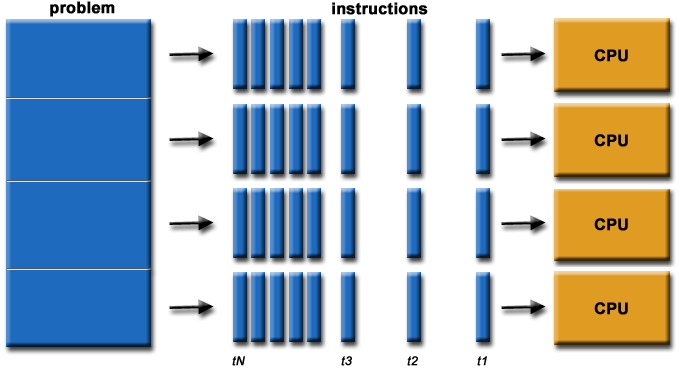
\includegraphics[width=0.8\textwidth]
		{pics/parallelProblem.png}
	\caption{Contoh masalah yang dikerjakan secara paralel}
	\label{fig:exmasalahparalel}
\end{figure}
\vspace{-0.8cm}
\begin{center}
{\small Sumber gambar: \citep{net.oxford}}
\end{center}

%-----------------------------------------------------------------------------%
\subsection{Klasifikasi X}
%-----------------------------------------------------------------------------%
Figure dalam enum dan dua sitasi sekaligus \citep{book.buyya,book.sterling-jones} :  
\begin{enumerate}
\item \bi{Bold Italic} \\
Penjelasan....... Untuk gambarannya dapat dilihat di Gambar \ref{fig:neumann}.

\begin{figure}
	\centering
	\includegraphics[height=0.65\textwidth,width=0.6\textwidth]
		{pics/neumann.pdf}
	\caption{Arsitektur klasik \f{von Neumann}}
	\label{fig:neumann}
\end{figure}
\vspace{-1.2cm}
\begin{center}
{\small Sumber gambar terinspirasi dari: \citep{buku.pressman}}
\end{center} 

\item \bi{Sesuatu banget} \\
Penjelasan.......
\end{enumerate}
\paragraph{}
%-----------------------------------------------------------------------------%
\section{\f{Section in Eng}}
%-----------------------------------------------------------------------------%
Hal pertama yang mungkin ditanyakan adalah bagaimana membuat huruf tercetak tebal, miring, atau memiliki garis bawah. 
Pada Texmaker, Anda bisa melakukan hal ini seperti halnya saat mengubah dokumen dengan LO Writer. 
Namun jika tetap masih tertarik dengan cara lain, ini dia: 

\begin{itemize}
	\item \bo{Bold} \\
		Gunakan perintah \bslash textbf$\lbrace\rbrace$ atau 
		\bslash bo$\lbrace\rbrace$. 
	\item \f{Italic} \\
		Gunakan perintah \bslash textit$\lbrace\rbrace$ atau 
		\bslash f$\lbrace\rbrace$. 
	\item \underline{Underline} \\
		Gunakan perintah \bslash underline$\lbrace\rbrace$.
	\item $\overline{Overline}$ \\
		Gunakan perintah \bslash overline. 
	\item $^{superscript}$ \\
		Gunakan perintah \bslash $\lbrace\rbrace$. 
	\item $_{subscript}$ \\
		Gunakan perintah \bslash \_$\lbrace\rbrace$. 
\end{itemize}

Perintah \bslash f dan \bslash bo hanya dapat digunakan jika package 
uithesis digunakan. 
%-----------------------------------------------------------------------------%
\subsection{Pengertian \f{Section in Eng}}
%-----------------------------------------------------------------------------%

%-----------------------------------------------------------------------------%
\subsection{Next Subsection \f{Section in Eng}}
%-----------------------------------------------------------------------------%

%-----------------------------------------------------------------------------%
\section{\f{Keatas lagi}}
%-----------------------------------------------------------------------------%
Contoh cite yang ga ada \cite{gaib}. Cite author \citeauthor{article.rebecca},cite tahun \citeyear{article.treese}, cite mention \cite{adin.experiment}, dan cite di akhir kalimat \citep{techreport.nist}.
%-----------------------------------------------------------------------------%
\subsection{\f{Masuk lagi}}
%-----------------------------------------------------------------------------%
Footnote example nih : MPICH \footnote{\url{http://www.mpich.org/}}, LAM/MPI \footnote{\url{http://www.lam-mpi.org/}}, dan OpenMPI \footnote{\url{www.open-mpi.org}} \citep{article.mcguire}. MPI-3 sedang dalam tahap perencanaan \footnote{\url{http://meetings.mpi-forum.org/MPI_3.0_main_page.php}}. Fungsi-fungsi tersebut berada di tabel \ref{tab:mpifund}. (Contoh tabel).

\begin{table}
	\centering
	\caption{Fungsi fundamental MPI}
	\label{tab:mpifund}
	\begin{tabular}{|c|c|c|}
	\hline
	\rowcolor{headertbl}	
	\hline No. & Nama Fungsi & Penjelasan \\ 
	\hline 1 & MPI\_Init & Memulai kode MPI \\ 
	\hline 2 & MPI\_Finalize & Mengakhiri kode MPI \\ 
	\hline 3 & MPI\_Comm\_size & Menentukan jumlah proses \\ 
	\hline 4 & MPI\_Comm\_rank & Menentukan label proses \\ 
	\hline 5 & MPI\_Send & Mengirim pesan \\ 
	\hline 6 & MPI\_Recv & Menerima pesan \\ 
	\hline
	\end{tabular}
\end{table}
\begin{center}
{\small Sumber tabel: taro sitasi disini, if i were u}
\end{center}